% Provenance (never printed): see sources/outline_sources.md (Year 2: effusive and explosive
% eruptions, eruptive styles, eruption columns, pyroclastic deposits, explosivity index,
% volcano monitoring).
% Curves from figdata/bachelor-2/eruptions.py (closed-system gas fraction, Cotopaxi Layer 5
% thinning, GVP frequency-size law, column height fits, Mogi uplift); exercise and problem
% values in the Book 4 scratch calculators calc/ch06.py and calc/ch06pb.py.
\chapter{As erupções vulcânicas}\label{ch:b2:eruptive-styles}

Em 15 de junho de 1991, o monte Pinatubo, nas Filipinas, lançou mais de cinco
quilômetros cúbicos de material; sua nuvem de cinzas subiu a
\qty{35}{km}, o cume desabou em uma \omterm{def:b2:eruptive-styles:caldera}{caldeira} de \qty{2.5}{km} de diâmetro, e os
vinte milhões de toneladas de dióxido de enxofre que ele injetou na estratosfera resfriaram o
globo inteiro em cerca de meio grau durante dois anos. Uma semana antes, o primeiro
\omterm{def:b2:magma-emplacement:magma}{magma} a chegar à superfície não tinha feito nada disso: tendo perdido a maior parte de seu
gás na subida, ele extravasou lentamente como um \omterm{def:b2:eruptive-styles:dome}{domo de lava}. No Kīlauea, no Havaí, a
erupção do Pu`u~`\=O`\=o derramou \qty{4.4}{km^3} de lava, volume comparável,
ao longo de trinta e cinco anos, em fontes e derrames que destruíram 215 construções
sem nunca erguer uma coluna de cinzas imponente. Mesma Terra, mesma física, três comportamentos: o que
os separa é a quantidade de gás que um \omterm{def:b2:magma-emplacement:magma}{magma} carrega, se esse gás pode deixar o
fundido tranquilamente e a velocidade com que o \omterm{def:b2:magma-emplacement:magma}{magma} sobe. Este capítulo acompanha uma erupção
desde as bolhas no conduto até a coluna acima da boca e os depósitos que ela
deixa, depois mede as erupções, conta-as e vigia os vulcões em busca dos
sinais de que uma delas se aproxima.
% ledger: usgs:pinatubo-1991, usgs:puuoo

\begin{recall}
\textbf{Dos volumes escolares}: um vulcão, sua boca e sua cratera, a câmara
magmática sob ele, a lava e as cinzas vulcânicas. \textbf{Do
\cref{ch:b2:magma-emplacement}}: os \omterm{def:b2:magma-emplacement:volatiles}{voláteis magmáticos}, sua exsolução abaixo da
pressão de saturação, a lei da raiz quadrada da solubilidade da água, $w = s\sqrt p$, com
$s \approx 0.34$ por cento por $\sqrt{\unit{MPa}}$ para o basalto e $0.44$ para o
riolito, e as viscosidades dos fundidos, separadas por dez ordens de grandeza.
\textbf{Dos livros de física}: a lei dos gases ideais $pV = nRT$; o empuxo;
a análise dimensional, que constrói a única combinação das grandezas dadas
que tem a dimensão da resposta; o alcance de um projétil, $v^2\sin 2\theta/g$,
sem resistência do ar. \textbf{Dos livros de matemática}: o processo de Poisson,
no qual eventos independentes a uma taxa constante $\lambda$ dão pelo menos um evento
em um tempo $t$ com probabilidade $1 - e^{-\lambda t}$; as retas de mínimos quadrados.
Do volume do primeiro ano: os terremotos e suas magnitudes.
\end{recall}

\section{Efusiva ou explosiva}

\begin{definition}[Erupções efusivas e explosivas, fragmentação]\label{def:b2:eruptive-styles:regimes}
Uma \emph{erupção efusiva}\index{erupção efusiva} é dominada pelo
extravasamento de lava, que escoa a partir da boca como um líquido coerente. Uma
\emph{erupção explosiva}\index{erupção explosiva} produz principalmente fragmentos,
cinzas, pedra-pomes e projéteis balísticos, carregados por gás em expansão. A \emph{fragmentação
do magma}\index{fragmentação do magma} é a ruptura de um fundido contínuo
contendo bolhas em um gás contínuo que carrega gotas e fragmentos de fundido;
ela transforma um escoamento efusivo em um escoamento explosivo.
\end{definition}
% ledger: usgs:glossary-ch6, cassidy18:fragmentation

O que impele a transição é o gás. Um \omterm{def:b2:magma-emplacement:magma}{magma} que sobe da profundidade carrega
água e dióxido de carbono dissolvidos; abaixo de sua pressão de saturação, os voláteis
saem da solução como bolhas, e as bolhas se expandem à medida que a pressão cai.
Se elas ficam no fundido, o gás logo preenche a maior parte do volume.

\begin{proposition}[Fração volumétrica de gás na desgaseificação em sistema fechado]\label{prop:b2:eruptive-styles:gas}
Suponha-se que um \omterm{def:b2:magma-emplacement:magma}{magma} contenha uma fração em massa $w_0$ de água, com solubilidade $w(p) =
s\sqrt p$, e suponha-se que a água exsolvida permaneça com o fundido como um gás
ideal à temperatura $T$. Abaixo da pressão de saturação $p_s = (w_0/s)^2$, um
quilograma de \omterm{def:b2:magma-emplacement:magma}{magma} contém $x = w_0 - s\sqrt p$ quilogramas de vapor, e a fração
volumétrica de gás é
\[
\phi(p) = \frac{V_g}{V_g + V_m}, \qquad V_g = \frac{x\,RT}{M p}, \qquad
V_m = \frac{1 - x}{\rho_m},
\]
onde $M = \qty{0.018}{kg/mol}$ é a massa molar da água e $\rho_m$ a densidade
do fundido.
\end{proposition}

\begin{proof}
Acima de $p_s$ o fundido pode conter toda a sua água e não existe gás. Abaixo de $p_s$ o
fundido conserva apenas sua solubilidade $s\sqrt p$, de modo que uma massa $x = w_0 - s\sqrt p$ por
quilograma de \omterm{def:b2:magma-emplacement:magma}{magma} é vapor. Esse vapor, $x/M$ mols, ocupa $xRT/(Mp)$ pela
lei dos gases ideais; os $1 - x$ quilogramas restantes de fundido ocupam $(1 - x)/\rho_m$.
Daí decorre a fração volumétrica.
\end{proof}
% ledger: moore98:h2o

Como $V_g$ cresce como $1/p$, a espuma incha mais depressa perto da superfície. A
figura abaixo acompanha um riolito com \qty{5}{\percent} de água e um basalto
com \qty{1}{\percent}. O riolito se satura a \qty{127}{MPa}, cerca de
\qty{5}{km} de profundidade; a \qty{10}{MPa} seu gás já preenche \qty{82}{\percent} do
volume. Em um modelo publicado de escoamento no conduto, o \omterm{def:b2:magma-emplacement:magma}{magma} se fragmenta quando o
gás preenche \qty{85}{\percent} de seu volume, nível que esse riolito atinge a
\qty{8.2}{MPa}, uns \qty{330}{m} abaixo da boca para um gradiente de pressão de
\qty{0.025}{MPa/m}. O basalto só se satura a \qty{8.7}{MPa} e atinge a
mesma espuma a \qty{1.8}{MPa}, a menos de cem metros da superfície.
% ledger: cassidy18:fragmentation, cassidy18:ascent

\begin{omfigure}
\centering
\begin{tikzpicture}
\begin{axis}[omrecord, width=0.82\linewidth, height=5.6cm, xmode=log,
  xmin=0.01, xmax=200, ymin=0, ymax=1,
  xlabel={pressão (\unit{MPa})}, ylabel={fração volumétrica de gás $\phi$},
  legend pos=south west, legend style={font=\scriptsize},
  tick label style={font=\scriptsize}, label style={font=\small}]
\addplot[very thick, red!70!black] table[x=p_MPa, y=rhyolite] {figdata/out/bachelor-2-eruptions-gas.dat};
\addlegendentry{riolito, \qty{5}{\percent} H$_2$O, \qty{850}{\celsius}}
\addplot[very thick, black, dashed] table[x=p_MPa, y=basalt] {figdata/out/bachelor-2-eruptions-gas.dat};
\addlegendentry{basalto, \qty{1}{\percent} H$_2$O, \qty{1200}{\celsius}}
\draw[densely dotted, thick, gray] (axis cs:0.01,0.85) -- (axis cs:200,0.85);
\node[anchor=north west, font=\scriptsize, inner sep=1pt] at (axis cs:0.012,0.835) {fragmentação em um modelo de conduto};
\end{axis}
\end{tikzpicture}
\par\smallskip{\small Fração volumétrica de vapor de água exsolvido em função da pressão
na desgaseificação em sistema fechado (\cref{prop:b2:eruptive-styles:gas}), com as leis de
solubilidade do \cref{ch:b2:magma-emplacement}. A pressão cai para a esquerda, à medida que o \omterm{def:b2:magma-emplacement:magma}{magma}
sobe; a linha pontilhada marca a fração de gás na qual um modelo de conduto publicado
fragmenta o \omterm{def:b2:magma-emplacement:magma}{magma}.}
\end{omfigure}
% ledger: moore98:h2o, cassidy18:fragmentation

Assim, um basalto também se fragmentaria se seu gás permanecesse nele; e em uma fonte de lava
havaiana é o que acontece, perto da boca. O que torna a maioria das erupções basálticas brandas é que
o gás não precisa ficar. Em um fundido de baixa viscosidade, as bolhas sobem através do
líquido, coalescem e escapam, e, uma vez que as bolhas se conectam em uma rede permeável,
o que ocorre em frações de gás entre \qty{30}{\percent} e \qty{78}{\percent}
nos experimentos, o gás escapa pelas paredes e pela boca sem arrastar o
fundido consigo: o \omterm{def:b2:magma-emplacement:magma}{magma} se desgaseifica em sistema aberto e chega à superfície como
lava. Um \omterm{def:b2:magma-emplacement:magma}{magma} viscoso retém suas bolhas e, em vez disso, se fragmenta, o fundido se quebrando
como vidro quando é estirado mais depressa do que consegue escoar. A taxa de ascensão decide
entre os dois tanto quanto a composição: em muitas erupções, a atividade efusiva
acompanha taxas de descompressão perto de \qty{0.0001}{MPa/s}, e as erupções explosivas
taxas perto de \qty{1}{MPa/s}, e uma variação da viscosidade do fundido de meia
unidade logarítmica, cerca de um fator três, pode fazer uma erupção passar de um regime ao
outro. O primeiro \omterm{def:b2:eruptive-styles:dome}{domo de lava} do Pinatubo e sua erupção paroxísmica uma semana depois
eram o mesmo \omterm{def:b2:magma-emplacement:magma}{magma}: o primeiro lote teve tempo de perder seu gás, o seguinte não.
% ledger: cassidy18:fragmentation, cassidy18:ascent, usgs:pinatubo-1991

A água externa faz o que faz o próprio gás do \omterm{def:b2:magma-emplacement:magma}{magma}. A água subterrânea, um lago ou o
mar que encontra o \omterm{def:b2:magma-emplacement:magma}{magma} se vaporiza instantaneamente, e a expansão da água
superaquecida estilhaça o \omterm{def:b2:magma-emplacement:magma}{magma}: experimentos mostram que mais de \qty{30}{\percent} do
calor disponível pode ser convertido em energia mecânica. Mesmo um \omterm{def:b2:magma-emplacement:magma}{magma} pobre em gás
pode então entrar em \omterm{def:b2:eruptive-styles:regimes}{erupção explosiva}.
% ledger: cassidy18:fragmentation

\section{Os estilos eruptivos}

Os vulcanólogos nomeiam as erupções a partir de exemplos clássicos. Os nomes descrevem o aspecto
de uma erupção, e passam gradualmente de um a outro; uma mesma erupção muitas vezes atravessa
vários estilos.

\begin{definition}[Estilos eruptivos]\label{def:b2:eruptive-styles:styles}
Em ordem de explosividade crescente, entre as erupções impelidas pelo próprio gás do \omterm{def:b2:magma-emplacement:magma}{magma}:
\begin{itemize}
\item uma \emph{erupção havaiana}\index{erupção havaiana} produz fontes de
lava basáltica muito fluida, com dezenas a centenas de metros de altura, que alimentam derrames de lava;
\item uma \emph{erupção estromboliana}\index{erupção estromboliana} é uma série de
explosões discretas que lançam fragmentos incandescentes de \omterm{def:b2:magma-emplacement:magma}{magma} basáltico a
andesito-basáltico até uns cem metros, sem coluna
sustentada;
\item uma \emph{erupção vulcaniana}\index{erupção vulcaniana} é uma explosão curta e violenta
de gás acumulado sob um tampão de lava solidificada, que estilhaça
o tampão e lança blocos e uma coluna escura de cinzas finas, tipicamente a partir de
\omterm{def:b2:magma-emplacement:magma}{magma} intermediário;
\item uma \emph{erupção pliniana}\index{erupção pliniana} é um jato sustentado de gás
e de \omterm{def:b2:magma-emplacement:magma}{magma} fragmentado, geralmente silícico, que alimenta uma coluna que sobe até a
estratosfera durante horas a dias e espalha um manto de pedra-pomes e cinzas sobre
milhares de quilômetros quadrados.
\end{itemize}
Quando a água externa impele a fragmentação, uma \emph{erupção
freatomagmática}\index{erupção freatomagmática} expele vapor junto com fragmentos
de \omterm{def:b2:magma-emplacement:magma}{magma} fresco, ao passo que uma \emph{erupção freática}\index{erupção freática} é uma
explosão impelida pelo vapor de água subterrânea ou superficial aquecida por \omterm{def:b2:magma-emplacement:magma}{magma} ou rocha quente,
que expele vapor e fragmentos de rocha mais antiga, mas nenhum \omterm{def:b2:magma-emplacement:magma}{magma} fresco.
\end{definition}
% ledger: nps:styles, usgs:glossary-ch6

Cada estilo tem suas erupções-tipo. O Pu`u~`\=O`\=o, no Kīlauea, foi havaiano durante a maior parte de
seus trinta e cinco anos e sessenta e um episódios, com fontes que tipicamente subiam
\qtyrange{10}{100}{m} e às vezes mais de \qty{500}{m}. O Stromboli, o
``farol do Mediterrâneo'', deu seu nome às explosões que constroem
cones de escória. Explosões vulcanianas sacudiram o Trident, no Alasca, de modo intermitente entre
1953 e 1974. O Vesúvio em 79 d.C., descrito por Plínio, o Jovem, deu seu nome às
erupções plinianas; o monte Santa Helena em 18 de maio de 1980 e o Novarupta em 1912, cuja
coluna subiu acima de \qty{30}{km} em uma erupção que durou quase três dias, são
exemplos modernos.
Os casos intermediários, com colunas abaixo de cerca de \qty{20}{km}, sustentadas mas instáveis,
são chamados subplinianos. Com água, uma \omterm{def:b2:eruptive-styles:styles}{erupção estromboliana} torna-se surtseiana,
nome dado a partir da erupção de 1963 de Surtsey, ao largo da Islândia, e constrói baixos
anéis de tufo e maares; uma pliniana torna-se freatopliniana. No Pinatubo, explosões de
vapor abriram três crateras no flanco norte em março e abril de 1991, dois
meses antes da erupção paroxísmica: eram freáticas.
% ledger: nps:styles, usgs:puuoo, usgs:glossary-ch6, usgs:pinatubo-deposits

\begin{definition}[Domo de lava]\label{def:b2:eruptive-styles:dome}
Um \emph{domo de lava}\index{domo de lava} é um monte de flancos íngremes de lava viscosa,
tipicamente dacito ou riolito, extrudido lentamente de uma boca e que se acumula sobre ela
em vez de escoar.
\end{definition}
% ledger: usgs:glossary-ch6

Os domos são o que um \omterm{def:b2:magma-emplacement:magma}{magma} viscoso produz quando perdeu seu gás: o primeiro
\omterm{def:b2:magma-emplacement:magma}{magma} do Pinatubo em junho de 1991, e o domo que cresceu na cratera do monte Santa Helena em
dezessete episódios entre 1980 e 1986 até \qty{267}{m} acima do fundo da cratera.
Um domo também pode ser o tampão sob o qual se prepara a explosão vulcaniana seguinte,
e seu colapso pode liberar a pressão sobre o \omterm{def:b2:magma-emplacement:magma}{magma} rico em gás abaixo dele. As
fotografias abaixo mostram os dois extremos da gama.
% ledger: usgs:pinatubo-1991, usgs:msh-dome, cassidy18:fragmentation

\begin{omfigure}
\centering
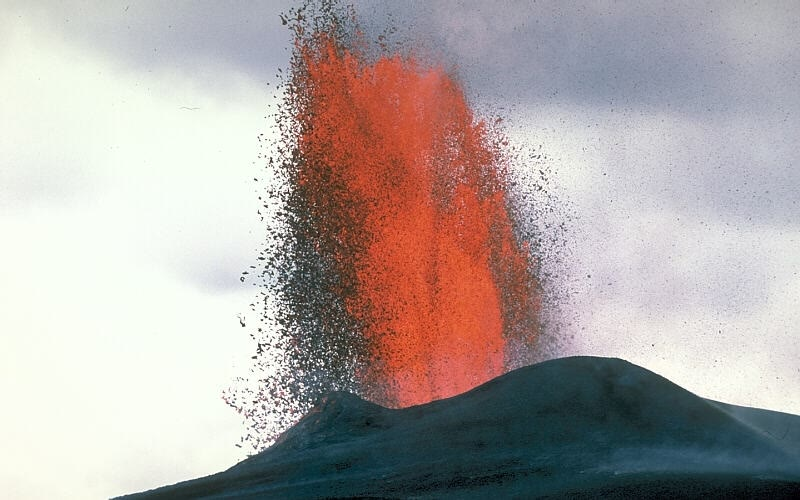
\includegraphics[height=4.3cm]{images/book4/b2-kilauea-fountain.jpg}\hfill
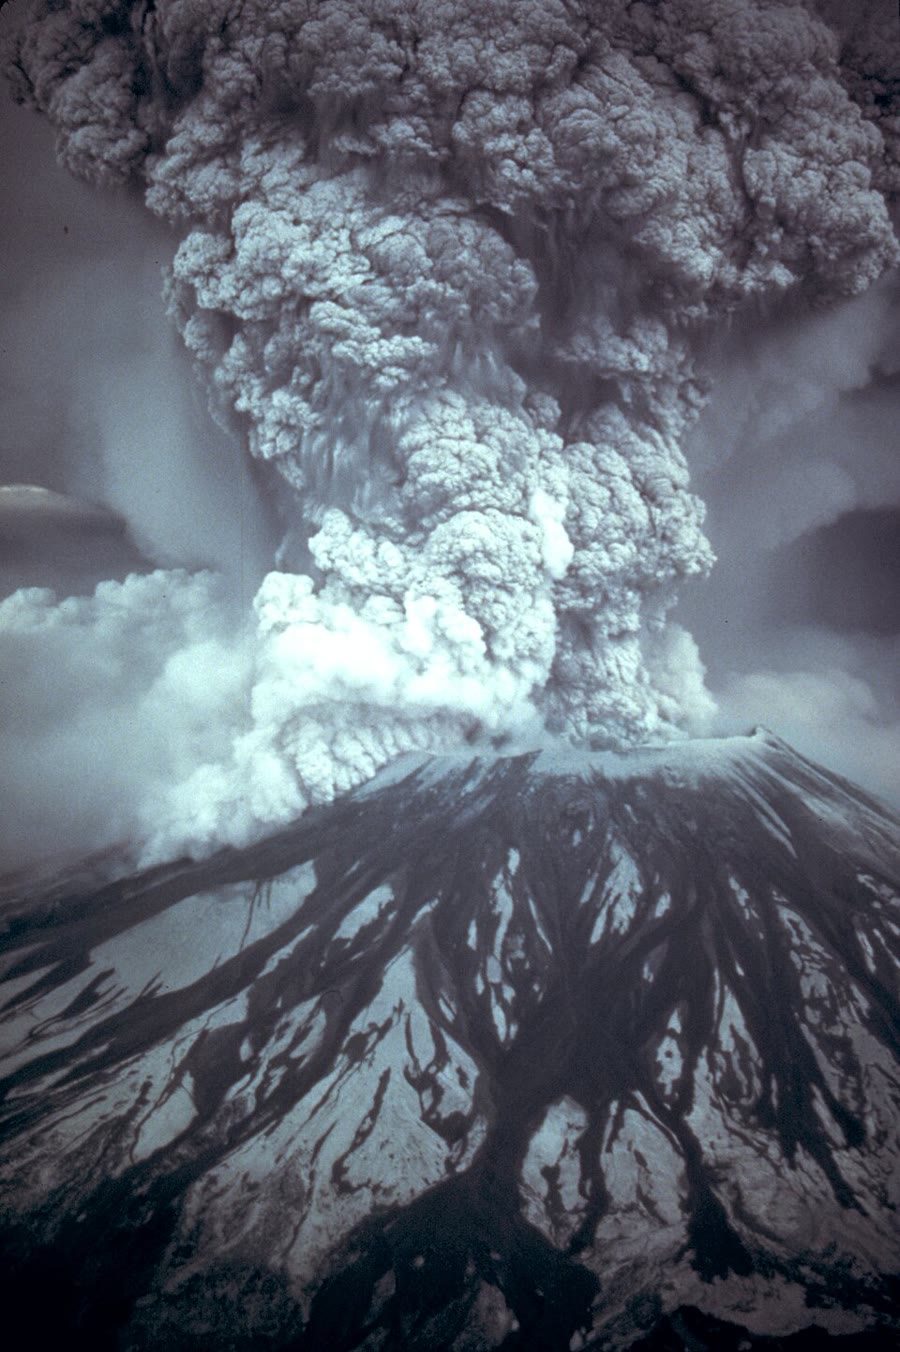
\includegraphics[height=4.3cm]{images/book4/b2-st-helens-column.jpg}\hfill
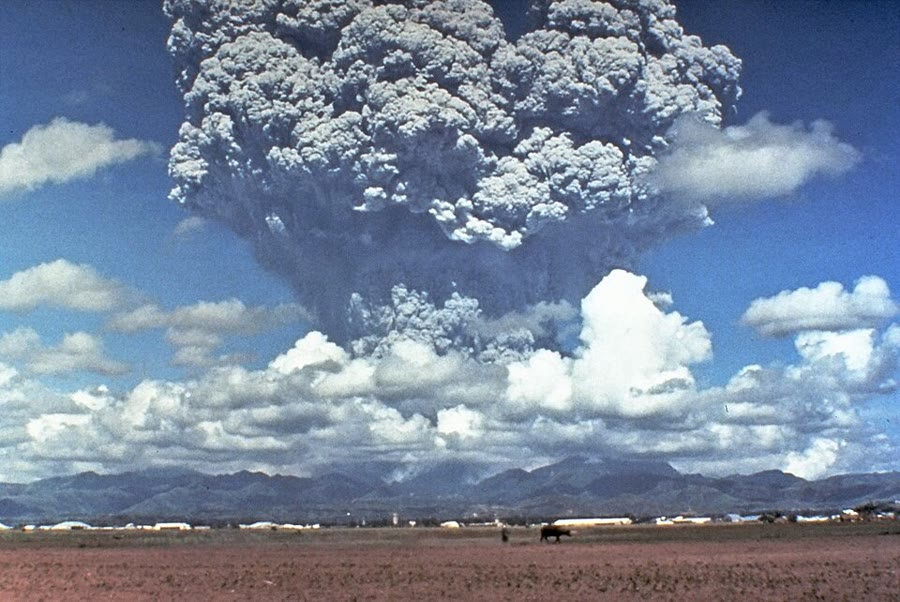
\includegraphics[height=4.3cm]{images/book4/b2-pinatubo-column.jpg}
\par\smallskip{\small À esquerda: uma fonte havaiana no cone do Pu`u~`\=O`\=o, no Kīlauea,
outubro de 1983 (J.\,D.~Griggs, USGS). No centro: a coluna pliniana do monte Santa Helena,
18 de maio de 1980 (Austin Post, USGS). À direita: a \omterm{def:b2:eruptive-styles:column}{coluna eruptiva} do monte Pinatubo em
12 de junho de 1991, três dias antes da erupção paroxísmica (Dave Harlow, USGS). As três
fotografias estão em domínio público.}
\end{omfigure}
% ledger: usgs:puuoo, usgs:msh-may18, usgs:pinatubo-1991

\section{As colunas eruptivas}

\begin{definition}[Coluna eruptiva]\label{def:b2:eruptive-styles:column}
Uma \emph{coluna eruptiva}\index{coluna eruptiva} é a massa ascendente de gás e de
fragmentos acima de uma boca explosiva. Ela tem três partes: um \emph{jato}, ou
região de impulso gasoso, no qual a mistura deixa a boca depressa, mas mais densa que o
ar, e sobe por sua quantidade de movimento; uma região \emph{convectiva}, na qual a mistura,
tendo englobado e aquecido ar suficiente para se tornar mais leve que o ambiente,
sobe por empuxo; e uma nuvem em \emph{guarda-chuva}, que se espalha lateralmente no
nível em que a densidade da coluna se iguala à da atmosfera.
\end{definition}
% ledger: usgs:glossary-ch6, nps:styles, aubry23:fits

\begin{omfigure}
\centering
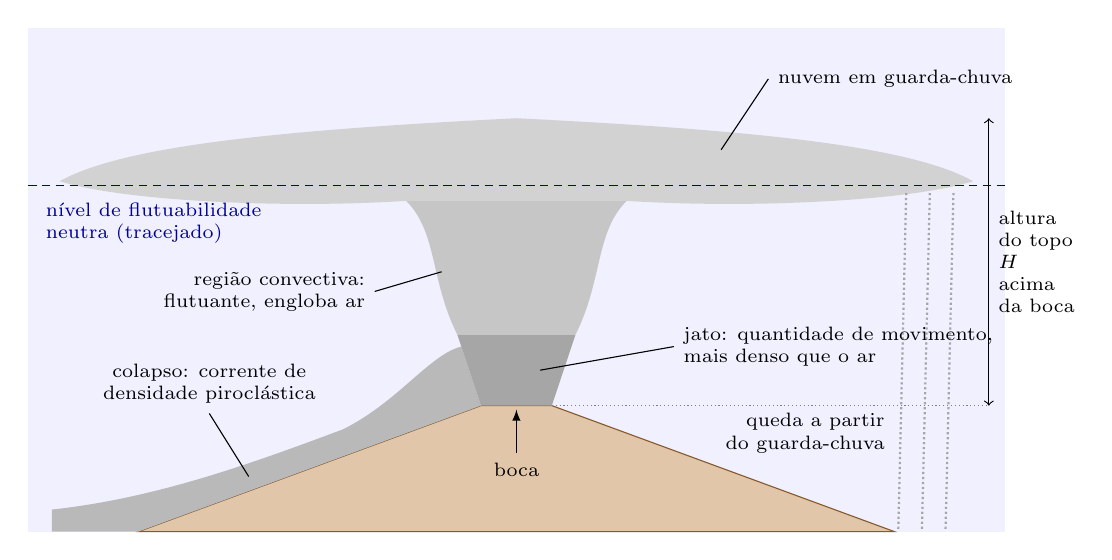
\begin{tikzpicture}[x=1cm, y=1cm, font=\scriptsize]
% atmosphere and ground
\fill[blue!6] (-6.2,0) rectangle (6.2,6.4);
% volcano
\fill[brown!45, draw=brown!70!black] (-4.8,0) -- (-0.45,1.6) -- (0.45,1.6) -- (4.8,0) -- cycle;
% collapse branch (left): a density current hugging the flank
\fill[gray!55] (-0.45,1.6) -- (-0.7,2.35) .. controls (-1.1,2.25) and (-1.5,1.65) .. (-2.2,1.3)
  .. controls (-3.4,0.85) and (-4.6,0.42) .. (-5.9,0.28) -- (-5.9,0) -- (-4.8,0) -- cycle;
% jet
\fill[gray!70] (-0.45,1.6) -- (0.45,1.6) -- (0.75,2.5) -- (-0.75,2.5) -- cycle;
% convective column
\fill[gray!45] (-0.75,2.5) .. controls (-1.1,3.2) and (-1.0,3.8) .. (-1.4,4.2)
  -- (1.4,4.2) .. controls (1.0,3.8) and (1.1,3.2) .. (0.75,2.5) -- cycle;
% umbrella
\fill[gray!35] (-1.4,4.2) .. controls (-3,4.1) and (-5,4.2) .. (-5.8,4.45)
  .. controls (-5,4.9) and (-3,5.1) .. (0,5.25) .. controls (3,5.1) and (5,4.9) .. (5.8,4.45)
  .. controls (5,4.2) and (3,4.1) .. (1.4,4.2) -- cycle;
\draw[densely dashed, blue!60!black] (-6.2,4.4) -- (6.2,4.4);
% fallout from the far end of the umbrella, down to the ground
\foreach \x in {4.95,5.25,5.55} {\draw[gray!70, densely dotted, thick] (\x,4.3) -- (\x-0.1,0.02);}
\draw[gray, densely dotted] (0.45,1.6) -- (6.0,1.6);
\draw[<->] (6.0,1.6) -- (6.0,5.25) node[midway, right, align=left] {altura\\do topo\\$H$\\acima\\da boca};
% labels
\node[anchor=north west, align=left, blue!60!black] at (-6.1,4.3) {nível de flutuabilidade\\neutra (tracejado)};
\draw (-0.95,3.3) -- (-1.8,3.05) node[left, align=right] {região convectiva:\\flutuante, engloba ar};
\draw (0.3,2.05) -- (2.0,2.35) node[right, align=left] {jato: quantidade de movimento,\\mais denso que o ar};
\draw (2.6,4.85) -- (3.2,5.75) node[right] {nuvem em guarda-chuva};
\node[anchor=east, align=right] at (4.8,1.25) {queda a partir\\do guarda-chuva};
\draw (-3.4,0.7) -- (-3.9,1.5) node[above, align=center] {colapso: corrente de\\densidade piroclástica};
\draw[-latex] (0,1.0) -- (0,1.55);
\node[anchor=north] at (0,1.0) {boca};
\end{tikzpicture}
\par\smallskip{\small Anatomia de uma \omterm{def:b2:eruptive-styles:column}{coluna eruptiva} (esquemático, fora de escala). À
direita, a coluna sobe através de suas três regiões e a nuvem em guarda-chuva
deixa cair \omterm{def:b2:eruptive-styles:tephra}{tefra} enquanto se espalha; à esquerda, parte do jato não conseguiu se tornar
flutuante e colapsa em uma \omterm{def:b2:eruptive-styles:pdc}{corrente de densidade piroclástica}.}
\end{omfigure}

A altura que uma coluna atinge depende sobretudo de quanto calor ela traz a cada
segundo, isto é, da vazão mássica eruptiva~$Q$. A análise dimensional dá a
forma da lei.

\begin{proposition}[Altura de uma pluma flutuante]\label{prop:b2:eruptive-styles:plume}
Se a altura do topo $H$ de uma pluma flutuante acima de uma fonte pontual estacionária depende apenas
do fluxo de empuxo $F$ da fonte (dimensão $\mathrm{m^4\,s^{-3}}$) e da
frequência de empuxo $N$ de uma atmosfera estavelmente estratificada (dimensão
$\mathrm{s^{-1}}$), então
\[
H = c\,F^{1/4}N^{-3/4}
\]
sendo $c$ uma constante adimensional. Como $F$ é proporcional ao fluxo de calor, e portanto
à vazão mássica eruptiva, $H \propto Q^{1/4}$ em uma atmosfera dada.
\end{proposition}

\begin{proof}
Escreva-se $H = c\,F^{\alpha}N^{\beta}$. Igualar os comprimentos dá $4\alpha = 1$; igualar os
tempos dá $-3\alpha - \beta = 0$. Logo $\alpha = 1/4$ e $\beta = -3/4$, e nenhuma
outra combinação de $F$ e $N$ tem a dimensão de um comprimento.
\end{proof}

A constante $c$ vem da rapidez com que a pluma engloba ar, que a teoria das plumas
trata com um coeficiente de entranhamento medido em experimentos; ela é admitida
aqui. As colunas reais não são fontes pontuais estacionárias em uma atmosfera calma, de modo que
os vulcanólogos ajustam a lei a erupções cuja altura e cuja vazão mássica foram
ambas medidas.
% ledger: aubry23:fits

\begin{proposition}[Altura da coluna e vazão mássica eruptiva]\label{prop:b2:eruptive-styles:mastin}
Para a altura do topo $H$ acima da boca em quilômetros e a vazão mássica eruptiva
$Q$ em quilogramas por segundo, a compilação de erupções bem documentadas dá
\[
H = 0.304\,Q^{0.241},
\]
e um conjunto de dados maior e independente, de 130 eventos, dá $H = 0.345\,Q^{0.226}$.
A dispersão é grande: o erro quadrático médio relativo sobre $H$ é de
\qtyrange{53}{60}{\percent}.
\end{proposition}
\admitted
% ledger: aubry23:fits

Os dois expoentes são próximos do $1/4$ da teoria das plumas. A figura abaixo mostra
os dois ajustes e as erupções de exemplo nas quais se baseiam os parâmetros de fonte usados pelos
centros de previsão de cinzas. Uma coluna de \qty{15}{km} de altura, como a do monte
Santa Helena, requer \qty{e7}{kg/s}, dez mil toneladas a cada segundo; dobrar a
altura requer quase dezoito vezes a vazão. Lida ao contrário, uma altura medida dá
a vazão, mas apenas a um fator de vários, porque $Q$ varia como $H^4$
(\cref{exo:b2:eruptive-styles:3}). Os vulcanólogos exprimem a vazão pela \emph{intensidade} $I =
\log_{10}Q + 3$, com $Q$ em quilogramas por segundo.
% ledger: mastin09:examples, aubry23:fits, brown14:record

\begin{omfigure}
\centering
\begin{tikzpicture}
\begin{axis}[omrecord, width=0.82\linewidth, height=6cm, xmode=log, ymode=log,
  xmin=1e3, xmax=1e9, ymin=1, ymax=60,
  xlabel={vazão mássica eruptiva $Q$ (\unit{kg/s})}, ylabel={altura do topo acima da boca (\unit{km})},
  ytick={1,2,5,10,20,50}, yticklabels={1,2,5,10,20,50},
  legend pos=north west, legend style={font=\scriptsize},
  tick label style={font=\scriptsize}, label style={font=\small}]
\addplot[very thick, black] table[x=Q, y=mastin] {figdata/out/bachelor-2-eruptions-column.dat};
\addlegendentry{$H = 0.304\,Q^{0.241}$}
\addplot[thick, red!70!black, dashed] table[x=Q, y=aubry] {figdata/out/bachelor-2-eruptions-column.dat};
\addlegendentry{$H = 0.345\,Q^{0.226}$}
\addplot[only marks, mark=*, mark size=1.8pt, blue!70!black]
  table[x=Q, y=H] {figdata/out/bachelor-2-eruptions-column-data.dat};
\addlegendentry{erupções de exemplo}
\begin{scope}[font=\tiny, inner sep=1.5pt]
\node[anchor=north west] at (axis cs:5e3,2) {Etna 2001};
\node[anchor=south east] at (axis cs:1e5,7) {Cerro Negro 1992};
\node[anchor=north west] at (axis cs:2e5,5) {Ruapehu 1996};
\node[anchor=east] at (axis cs:1e6,10) {Fuego 1974};
\draw[gray] (axis cs:3e6,10) -- (axis cs:2e7,4.5) node[anchor=west, black] {Soufrière Hills};
\draw[gray] (axis cs:4e6,11) -- (axis cs:2e7,6.5) node[anchor=west, black] {Spurr 1992};
\node[anchor=south east] at (axis cs:1e7,15) {Santa Helena 1980};
\node[anchor=south east, align=right] at (axis cs:1e8,25) {Santa Helena\\coignimbrito};
\end{scope}
\end{axis}
\end{tikzpicture}
\par\smallskip{\small Altura do topo das \omterm{def:b2:eruptive-styles:column}{colunas eruptivas} acima da boca em função da
vazão mássica eruptiva: o ajuste empírico de Mastin e colaboradores (2009), o ajuste de
Aubry e colaboradores (2023) a um conjunto de dados independente, e as erupções de exemplo
da primeira compilação (a nuvem coignimbrítica do monte Santa Helena subiu a partir de
\omterm{def:b2:eruptive-styles:pdc}{fluxos piroclásticos}, não da boca).}
\end{omfigure}
% ledger: aubry23:fits, mastin09:examples

Uma coluna também pode não conseguir subir. O jato deixa a boca mais denso que o ar; se
esgota sua quantidade de movimento antes de ter englobado ar suficiente para se tornar flutuante, por
exemplo porque seu teor de gás diminui, a coluna colapsa e a mistura
desce pelos flancos como uma corrente quente e densa. As colunas plinianas podem colapsar
dessa maneira, e no Pinatubo os \omterm{def:b2:eruptive-styles:pdc}{fluxos piroclásticos} de 1991 preencheram vales com
depósitos de até \qty{200}{m} de espessura.
% ledger: nps:styles, usgs:pinatubo-deposits

\section{Os produtos piroclásticos}

\begin{definition}[Tefra e piroclastos]\label{def:b2:eruptive-styles:tephra}
Um \emph{piroclasto}\index{piroclasto} é um fragmento produzido pela fragmentação
explosiva do \omterm{def:b2:magma-emplacement:magma}{magma} ou das rochas ao seu redor. \emph{Tefra}\index{tefra} é
o nome coletivo de todos os piroclastos lançados ao ar, qualquer que seja seu tamanho.
Por tamanho, os piroclastos mais finos que \qty{2}{mm} formam as cinzas vulcânicas; os de
\qtyrange{2}{64}{mm} são \emph{lápili}\index{lápili}; os maiores que
\qty{64}{mm} são blocos, se eram sólidos e angulosos ao serem ejetados, e uma
\emph{bomba vulcânica}\index{bomba vulcânica}, se estavam total ou parcialmente fundidos
e tomaram uma forma arredondada ou fusiforme em voo.
\end{definition}
% ledger: nps:pyroclast-sizes, usgs:glossary-ch6

A \omterm{def:b2:eruptive-styles:tephra}{tefra} cai da nuvem em guarda-chuva e da coluna, a sotavento, como um depósito de queda
que recobre o terreno: espesso perto da boca, mais delgado e mais fino longe dela. Sua
espessura é cartografada por \emph{isópacas}, linhas de igual espessura, e, em regra,
decresce exponencialmente com a distância. Como o vento estica as isópacas
em elipses, a distância é mais bem medida pela raiz quadrada da área que cada
isópaca encerra.
% ledger: usgs:ash-props, biass19:layer5

\begin{proposition}[Volume de um depósito que se adelgaça exponencialmente]\label{prop:b2:eruptive-styles:thinning}
Se a espessura de um depósito de queda decresce com a raiz quadrada $x = \sqrt A$
da área da isópaca como $T = T_0\,e^{-kx}$, seu volume aparente é
\[
V = \frac{2T_0}{k^2}.
\]
Metade desse volume fica além da isópaca $x_{1/2} = 1.678/k$.
\end{proposition}

\begin{proof}
Entre as isópacas de áreas $A$ e $A + dA$, o depósito tem volume $T\,dA$,
e $dA = 2x\,dx$. Assim, $V = \int_0^\infty T_0e^{-kx}\,2x\,dx = 2T_0/k^2$, por
integração por partes ($\int_0^\infty xe^{-kx}dx = 1/k^2$). O volume dentro de $x$
é $\frac{2T_0}{k^2}[1 - (1 + kx)e^{-kx}]$, que é metade do total quando $(1 +
u)e^{-u} = 1/2$ com $u = kx$, isto é, $u = 1.678$.
\end{proof}

Os depósitos reais se adelgaçam com duas ou mais inclinações, forte perto da boca e suave
longe, porque os \omterm{def:b2:eruptive-styles:tephra}{lápili} grossos caem depressa da coluna e as cinzas finas
derivam. Cada segmento é ajustado separadamente e a integral é calculada trecho por
trecho.

\begin{method}[Volume de um depósito de queda a partir de suas isópacas]\label{met:b2:eruptive-styles:volume}
Lance-se $\ln T$ em função de $\sqrt A$ para cada isópaca e ajuste-se uma reta a cada
série de pontos alinhados. Para dois segmentos, $T_0e^{-k_1x}$ dentro do ponto de cruzamento
$X$ das duas retas e o segundo além dele, o volume é
\[
V = \frac{2T_0}{k_1^2} + 2T_0e^{-k_1X}\left[\frac{k_2X + 1}{k_2^2} -
\frac{k_1X + 1}{k_1^2}\right]
\]
(\cref{exo:b2:eruptive-styles:10}). Converta-se o volume aparente em equivalente em rocha densa, o volume da
mesma massa sob forma de \omterm{def:b2:magma-emplacement:magma}{magma} sem bolhas, por $V_{\mathrm{DRE}} = V\rho_{\mathrm{deposit}}/\rho_{\mathrm{magma}}$.
\end{method}
% ledger: biass19:layer5, brown14:record

A figura abaixo aplica o método a uma queda de escória emitida pelo Cotopaxi, no
Equador, há cerca de \num{1200} anos. Dois segmentos se ajustam às seis isópacas, com
distâncias de meia espessura $\ln 2/k$ de \qty{1.9}{km} e \qty{5.0}{km} (o
estudo publicado, cujo ajuste difere ligeiramente, encontra \qty{1.9}{km} e
\qty{5.3}{km}), e o volume resulta em \qty{0.29}{km^3}, como nesse estudo. Mais de
\qty{40}{\percent} dele está no delgado segmento distal, e é por isso que as cinzas distais,
facilmente erodidas ou nunca cartografadas, pesam tanto no total. As cinzas recém-caídas
têm uma densidade aparente de \qtyrange{500}{1500}{kg/m^3}, bem abaixo da do
\omterm{def:b2:magma-emplacement:magma}{magma}, de modo que o equivalente em rocha densa é aproximadamente metade do volume aparente, ou menos.
% ledger: biass19:layer5, usgs:ash-props

\begin{omfigure}
\centering
\begin{tikzpicture}
\begin{axis}[omrecord, width=0.78\linewidth, height=5.6cm, ymode=log,
  xmin=0, xmax=30, ymin=2, ymax=2000,
  xlabel={$\sqrt{\text{área da isópaca}}$ (\unit{km})}, ylabel={espessura (\unit{cm})},
  ytick={2,5,10,20,50,100,200,500,1000,2000}, yticklabels={2,5,10,20,50,100,200,500,1000,2000},
  legend pos=north east, legend style={font=\scriptsize},
  tick label style={font=\scriptsize}, label style={font=\small}]
\addplot[thick, black, restrict x to domain=0:12] table[x=sqrtA_km, y=seg1] {figdata/out/bachelor-2-eruptions-thin-fit.dat};
\addlegendentry{segmento proximal, $k_1 = \qty{0.365}{km^{-1}}$}
\addplot[thick, red!70!black, dashed, restrict x to domain=5:30] table[x=sqrtA_km, y=seg2] {figdata/out/bachelor-2-eruptions-thin-fit.dat};
\addlegendentry{segmento distal, $k_2 = \qty{0.138}{km^{-1}}$}
\addplot[only marks, mark=*, mark size=2pt, blue!70!black] table[x=sqrtA_km, y=T_cm] {figdata/out/bachelor-2-eruptions-thin-data.dat};
\addlegendentry{isópacas}
\end{axis}
\end{tikzpicture}
\par\smallskip{\small Adelgaçamento da queda de escória da Camada~5 do Cotopaxi (Equador),
com cerca de \num{1200} anos: espessuras das isópacas segundo Biass, Bonadonna e
Houghton (2019) em função da raiz quadrada da área que cada isópaca encerra (a
escala vertical é logarítmica). Dois segmentos exponenciais, ajustados às duas
isópacas proximais e às quatro distais, cruzam-se em $\sqrt A = \qty{8.6}{km}$;
integrados, dão um volume aparente de \qty{0.29}{km^3}.}
\end{omfigure}
% ledger: biass19:layer5

Nem toda \omterm{def:b2:eruptive-styles:tephra}{tefra} cai do céu. Quando uma coluna colapsa, um domo desmorona ou uma
explosão lateral rasga o flanco de um vulcão, a mistura quente corre rente ao
solo.

\begin{definition}[Correntes de densidade piroclásticas]\label{def:b2:eruptive-styles:pdc}
Uma \emph{corrente de densidade piroclástica}\index{corrente de densidade piroclástica} é uma
mistura de gás quente e \omterm{def:b2:eruptive-styles:tephra}{piroclastos}, rente ao solo, que escoa encosta abaixo ou para fora
porque é mais densa que o ar. Um \emph{fluxo piroclástico}\index{fluxo piroclástico}
é uma corrente concentrada de fragmentos de rocha, cinzas e gás, geralmente a
\qtyrange{200}{700}{\celsius}, que se move a dezenas de metros por segundo; um
\emph{surge piroclástico}\index{surge piroclástico} é uma nuvem mais diluída de cinzas,
rocha e gás, a várias centenas de graus, que se move à velocidade de um vento de
furacão. Um \emph{ignimbrito}\index{ignimbrito} é a rocha depositada pelas correntes de
densidade piroclásticas, que pode ser soldada por seu próprio calor.
\end{definition}
% ledger: usgs:glossary-ch6

Em 18 de maio de 1980, o colapso do flanco norte do monte Santa Helena, o maior
deslizamento de terra da história registrada, com cerca de \qty{2.8}{km^3}, descobriu o \omterm{def:b2:magma-emplacement:magma}{magma} e
liberou uma explosão lateral que varreu cerca de \qty{600}{km^2} a até
\qty{480}{km/h}; \omterm{def:b2:eruptive-styles:pdc}{fluxos piroclásticos} de pelo menos \qty{700}{\celsius} chegaram então a
\qty{8}{km} da cratera. Os fluxos do Pinatubo de 1991 ainda estavam a até
\qty{500}{\celsius} em seu interior cinco anos depois.
% ledger: usgs:msh-may18, usgs:msh-flows, usgs:msh-reach, usgs:pinatubo-deposits

\begin{definition}[Lahar]\label{def:b2:eruptive-styles:lahar}
Um \emph{lahar}\index{lahar} é uma mistura rápida de água e detritos vulcânicos
que desce por um vale fluvial, com uma consistência que vai da água barrenta
ao concreto úmido. Os lahars se formam quando correntes piroclásticas derretem neve e gelo, quando
chuvas fortes caem sobre depósitos vulcânicos soltos, quando um lago represado por depósitos
vulcânicos se rompe, ou a partir de uma avalanche de detritos.
\end{definition}
% ledger: usgs:glossary-ch6

Os \omterm{def:b2:eruptive-styles:lahar}{lahars} sobrevivem às erupções. Em torno do Pinatubo, as chuvas de monção e de tufão transformaram
as cinzas de 1991 em \omterm{def:b2:eruptive-styles:lahar}{lahars} durante anos, e eles causaram mais destruição que a
própria erupção.
% ledger: usgs:pinatubo-lahars

\begin{definition}[Caldeira]\label{def:b2:eruptive-styles:caldera}
Uma \emph{caldeira}\index{caldeira} é uma grande depressão vulcânica em forma de bacia,
com \qtyrange{2}{50}{km} de diâmetro e muito mais larga que qualquer boca em seu interior, formada pelo
colapso do terreno em um reservatório magmático raso que uma erupção
esvaziou em parte.
\end{definition}
% ledger: usgs:glossary-ch6

As \omterm{def:b2:eruptive-styles:caldera}{caldeiras} do Pinatubo e do Novarupta têm ambas cerca de \qty{2.5}{km} de diâmetro, no
extremo inferior da gama. Uma \omterm{def:b2:eruptive-styles:caldera}{caldeira} difere de uma cratera, que é menor e escavada por explosões.
% ledger: usgs:pinatubo-1991, nps:styles, usgs:glossary-ch6

\section{Medir e contar as erupções}

\begin{definition}[Índice de explosividade vulcânica]\label{def:b2:eruptive-styles:vei}
O \emph{índice de explosividade vulcânica}\index{índice de explosividade vulcânica} (VEI) é
um inteiro de 0 a 8 que mede o tamanho de uma erupção, principalmente pelo
volume aparente de sua \omterm{def:b2:eruptive-styles:tephra}{tefra}: VEI~0 para menos de \qty{e4}{m^3}, VEI~1 até
\qty{e6}{m^3}, depois um degrau a cada fator dez, até VEI~8 além de
\qty{e12}{m^3}, \qty{1000}{km^3}. A altura da coluna e as descrições da erupção
são usadas quando o volume não é conhecido. Uma erupção não explosiva tem VEI~0,
qualquer que seja o volume de sua lava.
\end{definition}
% ledger: usgs:vei-criteria, usgs:msh-comparisons

\begin{table}[ht]
\centering
\small
\begin{tabular}{llll}
\hline
VEI & volume aparente de \omterm{def:b2:eruptive-styles:tephra}{tefra} (\unit{m^3}) & altura da coluna (\unit{km}) & estilo usual \\
\hline
0 & $< 10^{4}$ & $< 0.1$ & havaiano \\
1 & $10^{4}$--$10^{6}$ & 0.1--1 & havaiano, estromboliano \\
2 & $10^{6}$--$10^{7}$ & 1--5 & estromboliano, vulcaniano \\
3 & $10^{7}$--$10^{8}$ & 3--15 & vulcaniano \\
4 & $10^{8}$--$10^{9}$ & 10--25 & vulcaniano, pliniano \\
5 & $10^{9}$--$10^{10}$ & $> 25$ & pliniano \\
6 & $10^{10}$--$10^{11}$ & $> 25$ & pliniano \\
7 & $10^{11}$--$10^{12}$ & $> 25$ & pliniano \\
8 & $> 10^{12}$ & $> 25$ & pliniano \\
\hline
\end{tabular}
\caption{Critérios do \omterm{def:b2:eruptive-styles:vei}{índice de explosividade vulcânica} (segundo Newhall e Self, 1982).}
\label{tab:b2:eruptive-styles:vei}
\end{table}
% ledger: usgs:vei-criteria

O índice é logarítmico como a magnitude de um terremoto, mas mais grosseiro. O monte
Santa Helena em 1980, com \qty{1.3}{km^3} de cinzas, foi classificado como VEI~5, ``mas por pouco'';
o Pinatubo em 1991, como VEI~6; o Tambora em 1815, que expeliu de trinta a oitenta
vezes mais cinzas que o monte Santa Helena, como VEI~7, a maior \omterm{def:b2:eruptive-styles:regimes}{erupção explosiva}
dos tempos históricos. Para o trabalho quantitativo, os vulcanólogos preferem a
\emph{magnitude} $M = \log_{10}m - 7$, sendo $m$ a massa emitida em quilogramas, que
evita a densidade aparente do depósito, e a intensidade definida acima para a
vazão.
% ledger: usgs:msh-1980-ash, usgs:msh-comparisons, data:b4-gvp-eruptions, brown14:record

As pequenas erupções são frequentes e as grandes, raras. O catálogo global das
erupções do Holoceno torna a relação quantitativa, desde que se levem em conta suas
lacunas: uma erupção só está no catálogo se alguém a registrou ou encontrou seu
depósito, e as pequenas erupções longe de observadores, ou com mais de alguns séculos,
muitas vezes passaram despercebidas. O registro das grandes erupções é completo há mais tempo que
o das pequenas. No painel da esquerda da figura abaixo, as erupções de cada
tamanho registradas desde 1500 se acumulam com o tempo; um registro completo a uma taxa constante
seguiria a diagonal. As erupções de VEI~3 ou mais se concentram no último
século, porque a maioria das anteriores nunca foi registrada; o registro de VEI~6
fica perto da diagonal.
% ledger: data:b4-gvp-eruptions, brown14:record

\begin{dated}{2026}
O catálogo do Global Volcanism Program lista \num{7747} erupções confirmadas do Holoceno
com um VEI. Contando do início de uma janela até o fim de 2024, houve
399 erupções de VEI~3 ou mais desde 1950, 95 de VEI~4 ou mais desde 1900,
22 de VEI~5 ou mais desde 1800 e 8 de VEI~6 ou mais desde 1500 (a mais
recente, o Pinatubo em 1991). Só duas erupções de VEI~7 estão registradas desde o ano
1000: o Rinjani em 1257 e o Tambora, cuja erupção começou em 1812 e culminou em
1815.
\end{dated}
% ledger: data:b4-gvp-eruptions, usgs:msh-comparisons

\begin{proposition}[Lei frequência--tamanho das erupções]\label{prop:b2:eruptive-styles:frequency}
Seja $\lambda_v$ o número médio de erupções de VEI $\ge v$ por ano na Terra,
cada um estimado sobre uma janela na qual seu registro é quase completo (desde 1950
para $v = 3$, 1900 para $v = 4$, 1800 para $v = 5$, 1500 para $v = 6$). Então, por mínimos
quadrados,
\[
\log_{10}\lambda_v = 3.28 - 0.85\,v .
\]
Cada degrau de VEI é cerca de sete vezes mais raro que o anterior.
\end{proposition}
% ledger: data:b4-gvp-eruptions

A lei é empírica, um ajuste a quatro pontos, e seu expoente depende das
janelas escolhidas; ela prevê uma erupção de VEI~7 ou mais a cada \num{470} anos,
perto das duas dos últimos mil anos, que não foram usadas para ajustá-la. Como
as erupções são quase independentes umas das outras, elas se comportam como um processo de
Poisson, e a probabilidade de pelo menos uma erupção de VEI $\ge v$ em $t$ anos
é $1 - e^{-\lambda_vt}$ (problema de fim de semana).
% ledger: data:b4-gvp-eruptions

\begin{omfigure}
\centering
\begin{tikzpicture}
\begin{axis}[omrecord, name=cum, width=0.47\linewidth, height=5.6cm,
  xmin=1500, xmax=2024, ymin=0, ymax=1,
  xlabel={ano}, ylabel={fração registrada desde 1500},
  xtick={1500,1600,1700,1800,1900,2000}, x tick label style={/pgf/number format/1000 sep={}},
  legend pos=north west, legend style={font=\tiny},
  tick label style={font=\scriptsize}, label style={font=\small}]
\addplot[thick, gray, densely dotted, domain=1500:2024, samples=2] {(x - 1500)/524};
\addlegendentry{taxa constante}
\addplot[thick, blue!70!black] table[x=year, y=f3] {figdata/out/bachelor-2-eruptions-vei-cumul.dat};
\addlegendentry{VEI $\ge 3$}
\addplot[thick, black, dashed] table[x=year, y=f4] {figdata/out/bachelor-2-eruptions-vei-cumul.dat};
\addlegendentry{VEI $\ge 4$}
\addplot[thick, orange!80!black, dashdotted] table[x=year, y=f5] {figdata/out/bachelor-2-eruptions-vei-cumul.dat};
\addlegendentry{VEI $\ge 5$}
\addplot[thick, red!70!black, const plot] table[x=year, y=f6] {figdata/out/bachelor-2-eruptions-vei-cumul.dat};
\addlegendentry{VEI $\ge 6$}
\end{axis}
\begin{axis}[omrecord, at={(cum.east)}, anchor=west, xshift=1.9cm,
  width=0.47\linewidth, height=5.6cm, ymode=log,
  xmin=2.5, xmax=7.5, ymin=1e-3, ymax=20,
  xlabel={VEI $v$}, ylabel={erupções de VEI $\ge v$ por ano},
  xtick={3,4,5,6,7},
  tick label style={font=\scriptsize}, label style={font=\small}]
\addplot[thick, black] table[x=vei, y=rate] {figdata/out/bachelor-2-eruptions-vei-fit.dat};
\addplot[only marks, mark=*, mark size=2pt, blue!70!black] table[x=vei, y=rate] {figdata/out/bachelor-2-eruptions-vei-rate.dat};
\addplot[only marks, mark=o, mark size=2.4pt, red!70!black] table[x=vei, y=rate] {figdata/out/bachelor-2-eruptions-vei-rate7.dat};
\node[font=\tiny, anchor=south west] at (axis cs:3.05,6) {desde 1950};
\node[font=\tiny, anchor=south west] at (axis cs:4.05,0.8) {desde 1900};
\node[font=\tiny, anchor=south west] at (axis cs:5.05,0.1) {desde 1800};
\node[font=\tiny, anchor=south west] at (axis cs:6.05,0.016) {desde 1500};
\node[font=\tiny, anchor=east, red!70!black] at (axis cs:6.85,0.00195) {desde 1000};
\end{axis}
\end{tikzpicture}
\par\smallskip{\small À esquerda: completude do registro global. Para cada tamanho,
a fração das erupções registradas entre 1500 e 2024 que já tinham
ocorrido em um dado ano; um registro completo a uma taxa constante seguiria a
diagonal pontilhada. À direita: taxa anual das erupções de VEI $\ge v$, cada uma contada sobre
sua própria janela, e a reta de mínimos quadrados da
\cref{prop:b2:eruptive-styles:frequency}; o círculo vazio, VEI $\ge 7$ desde o ano
1000, não foi usado no ajuste. Dados: Global Volcanism Program, Volcanoes of the
World.}
\end{omfigure}
% ledger: data:b4-gvp-eruptions

\section{Vigiar os vulcões}

O \omterm{def:b2:magma-emplacement:magma}{magma} não chega à superfície sem aviso. Ele precisa romper a rocha para abrir seu
caminho, empurra o solo para cima ao se acumular, libera gás à medida que a pressão
sobre ele cai e aquece o solo. Os observatórios vulcanológicos monitoram os quatro sinais.

\emph{Sismicidade.} O \omterm{def:b2:magma-emplacement:magma}{magma} que se move pela crosta rompe a rocha e desencadeia enxames
de pequenos terremotos. Antes de 18 de maio de 1980, o monte Santa Helena produziu mais de
\num{10000} deles em dois meses; o Pinatubo produziu milhares entre abril e
junho de 1991, a partir de \omterm{def:b2:magma-emplacement:magma}{magma} que subia de mais de \qty{32}{km} de profundidade. As magnitudes
e os momentos sísmicos do volume do primeiro ano se aplicam sem mudança; o que difere são as
fontes, fraturas que se abrem e condutos cheios de fluido que ressoam, além de falhas.
% ledger: usgs:msh-lead-up, usgs:pinatubo-deposits

\emph{Deformação.} Um reservatório que se enche infla e levanta o solo acima
dele. O nivelamento, os inclinômetros e o posicionamento por satélite medem o soerguimento; a interferometria de radar por satélite o cartografa sobre vulcões
inteiros, uma técnica que o volume do terceiro ano desta série explica. O modelo mais
simples trata o reservatório como uma pequena esfera.

\begin{proposition}[Fonte de Mogi]\label{prop:b2:eruptive-styles:mogi}
Uma pequena fonte esférica à profundidade $z_0$ em um semiespaço elástico homogêneo
de coeficiente de Poisson $\nu$, cujo volume varia de $\Delta V$, uma
\emph{fonte de Mogi}\index{fonte de Mogi}, levanta a superfície à distância horizontal $r$
de
\[
u_z(r) = \frac{(1 - \nu)\,\Delta V}{\pi}\,\frac{z_0}{(r^2 + z_0^2)^{3/2}} .
\]
\end{proposition}
\admitted
% ledger: dmodels:mogi

O soerguimento é máximo acima da fonte, $u_z(0) = (1 - \nu)\Delta V/(\pi z_0^2)$, e
cai à metade desse valor em $r = z_0\sqrt{2^{2/3} - 1} = 0.766\,z_0$: a largura do
abaulamento dá a profundidade da fonte, e sua altura dá então a variação de
volume. Como só $\Delta V$ intervém, a pressão no reservatório e seu tamanho
não podem ser separados, de modo que são variações de volume, e não pressões, o que os geodesistas
relatam. A fórmula é o primeiro termo de uma solução exata para uma esfera de raio
$a$; a correção é de \qty{12}{\percent} quando $a = z_0/2$ e de \qty{3}{\percent}
quando $a = z_0/3$.
% ledger: dmodels:mogi

\begin{omfigure}
\centering
\begin{tikzpicture}
\begin{axis}[omrecord, width=0.78\linewidth, height=5.2cm,
  xmin=-12, xmax=12, ymin=0, ymax=65,
  xlabel={distância horizontal à fonte (\unit{km})}, ylabel={soerguimento (\unit{mm})},
  legend pos=north east, legend style={font=\scriptsize},
  tick label style={font=\scriptsize}, label style={font=\small}]
\addplot[very thick, black] table[x=r_km, y=z2] {figdata/out/bachelor-2-eruptions-mogi.dat};
\addlegendentry{fonte a \qty{2}{km}}
\addplot[very thick, red!70!black, dashed] table[x=r_km, y=z4] {figdata/out/bachelor-2-eruptions-mogi.dat};
\addlegendentry{fonte a \qty{4}{km}}
\draw[<->, thin] (axis cs:-1.532,29.8) -- (axis cs:1.532,29.8) node[midway, below, font=\tiny] {$2\times 0.766\,z_0$};
\end{axis}
\end{tikzpicture}
\par\smallskip{\small Soerguimento da superfície acima de uma \omterm{prop:b2:eruptive-styles:mogi}{fonte de Mogi} cujo volume cresce de
\qty{e6}{m^3} ($\nu = 0.25$), a duas profundidades. Com o dobro da profundidade, o abaulamento é quatro
vezes mais baixo e duas vezes mais largo; a seta marca a largura total a meia altura
do mais raso.}
\end{omfigure}
% ledger: dmodels:mogi

\emph{Gás e calor.} À medida que o \omterm{def:b2:magma-emplacement:magma}{magma} sobe e se desgaseifica, o fluxo de dióxido de enxofre na
superfície cresce, e ele é medido a partir do solo, de aeronaves e de
satélites; o Pinatubo emitiu muitos milhares de toneladas dele nas semanas anteriores à sua erupção.
O calor do \omterm{def:b2:magma-emplacement:magma}{magma} raso aparece nas imagens térmicas do solo e da boca.
% ledger: usgs:pinatubo-deposits

A partir desses dados, um observatório fixa um nível de alerta. Nos Estados Unidos, o
nível de alerta vulcânico em terra, em uso desde 2006, tem quatro degraus, NORMAL,
ADVISORY, WATCH e WARNING, e um código de cores paralelo para a aviação, de GREEN a RED,
avisa as aeronaves sobre as cinzas. Não há limiares fixos: cada mudança é decidida pelos
cientistas do observatório a partir de todos os dados de monitoramento, do comportamento
passado do vulcão e do que se sabe sobre os processos em curso. A previsão continua
probabilística: quando uma erupção vai começar e qual será seu tamanho são difíceis de
prever. No Pinatubo, a previsão de 1991 permitiu que as pessoas que viviam perto do
vulcão se afastassem a tempo e salvou pelo menos \num{5000} vidas. O modo como tais previsões
entram nas decisões sobre perigo e risco pertence ao \cref{ch:b2:geological-hazards}.
% ledger: hvo:alert-levels, usgs:pinatubo-1991

\begin{inthefield}[Em um observatório vulcanológico]
\begin{minipage}[t]{0.6\linewidth}\vspace{0pt}
Um observatório vigia seus vulcões dia e noite. Os sismômetros nos flancos
enviam seus sinais por rádio a telas nas quais cientistas de plantão procuram enxames,
o tremor, a vibração contínua do fluido que se move em um conduto, e mudanças
na profundidade dos eventos. Estações de posicionamento e inclinômetros registram a
inflação do solo, câmeras a boca, espectrômetros de gás o fluxo de dióxido de
enxofre na pluma. Quando um sinal se afasta do ruído de fundo do vulcão, os
cientistas o comparam com episódios anteriores, reúnem-se e decidem se o nível de
alerta deve mudar; o aviso que emitem diz o que se observa e o que pode
seguir, sem exagerar nem um nem outro.
\end{minipage}\hfill
\begin{minipage}[t]{0.36\linewidth}\vspace{0pt}
\centering
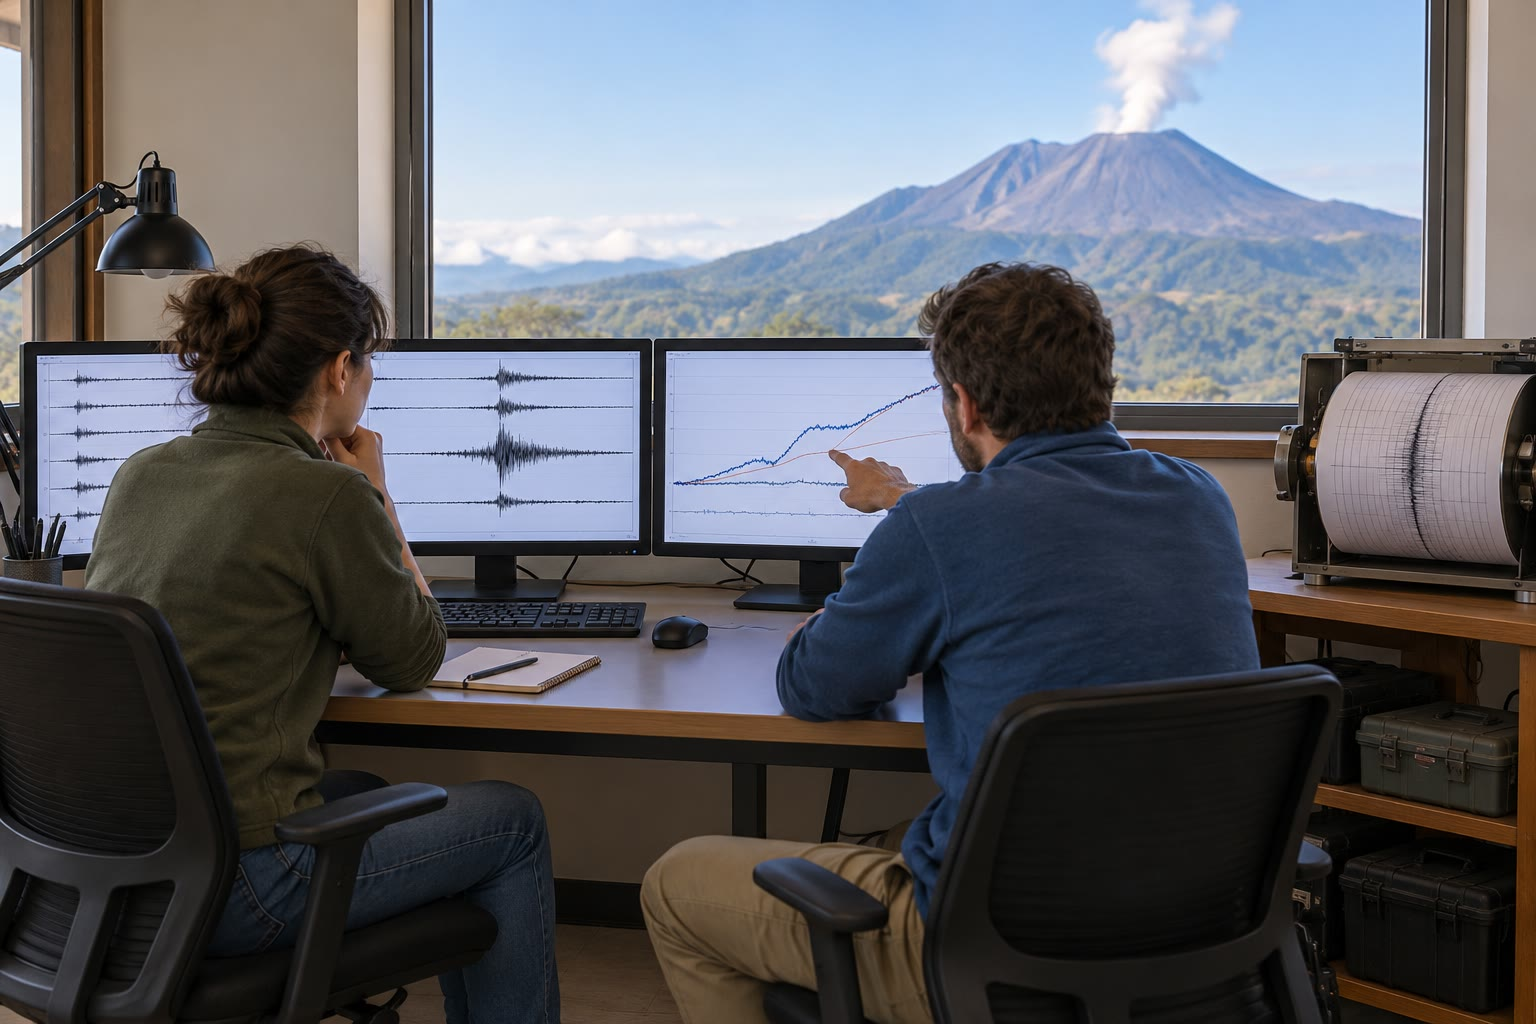
\includegraphics[width=\linewidth]{images/book4/ai/b2-volcano-observatory.jpg}
\par\smallskip{\scriptsize Cientistas examinam registros sísmicos em um observatório
vulcanológico (ilustração gerada por IA).}
\end{minipage}
\end{inthefield}
% ledger: hvo:alert-levels

\section{Exercícios}

\begin{exercise}[$\star$]\label{exo:b2:eruptive-styles:1}
Dê o VEI indicado apenas pelo volume aparente de \omterm{def:b2:eruptive-styles:tephra}{tefra} para: (a) as cinzas do
monte Santa Helena, 18 de maio de 1980, \qty{1.3}{km^3}; (b) a queda da Camada~5 do Cotopaxi,
\qty{0.29}{km^3}; (c) uma pequena erupção de \qty{2e6}{m^3}. (d) O material
expelido pelo Pinatubo em 1991 é dado como ``mais de \qty{5}{km^3}'', mas a
erupção é classificada como VEI~6. Que volume aparente essa classificação implica, no mínimo?
\end{exercise}
% ledger: usgs:vei-criteria, usgs:msh-1980-ash, biass19:layer5, usgs:pinatubo-1991

\begin{exercise}[$\star$]\label{exo:b2:eruptive-styles:2}
Dê o nome de cada \omterm{def:b2:eruptive-styles:tephra}{piroclasto}: (a) um fragmento de vidro de \qty{0.5}{mm} de comprimento; (b) um fragmento
de pedra-pomes de \qty{3}{cm} de diâmetro; (c) um pedaço anguloso de lava antiga de \qty{20}{cm}
de diâmetro; (d) um coágulo fusiforme de \qty{8}{cm} de comprimento com as pontas torcidas.
\end{exercise}
% ledger: nps:pyroclast-sizes

\begin{exercise}[$\star$]\label{exo:b2:eruptive-styles:3}
Com $H = 0.304\,Q^{0.241}$ ($H$ em quilômetros acima da boca, $Q$ em
\unit{kg/s}): (a) calcule $H$ para $Q = \qty{e6}{kg/s}$ e \qty{e8}{kg/s};
(b) calcule a vazão mássica eruptiva implicada por uma coluna de \qty{35}{km} de altura, e sua
intensidade $I = \log_{10}Q + 3$; (c) por que fator $Q$ varia se a altura medida
for \qty{20}{\percent} alta demais?
\end{exercise}
% ledger: aubry23:fits, brown14:record

\begin{exercise}[$\star$]\label{exo:b2:eruptive-styles:4}
A queda da Camada~5 do Cotopaxi tem um volume aparente de \qty{0.29}{km^3}. Tomando uma
densidade aparente de \qty{1000}{kg/m^3} para o depósito e de \qty{2500}{kg/m^3} para o
\omterm{def:b2:magma-emplacement:magma}{magma}, calcule seu volume equivalente em rocha densa, sua massa e sua magnitude
$M = \log_{10}m - 7$.
\end{exercise}
% ledger: biass19:layer5, brown14:record

\begin{exercise}[$\star\star$]\label{exo:b2:eruptive-styles:5}
Um depósito de queda tem \qty{40}{cm} de espessura na isópaca de $\sqrt A = \qty{5}{km}$
e \qty{10}{cm} na de $\sqrt A = \qty{15}{km}$, e se adelgaça segundo uma única
exponencial. Calcule $k$, $T_0$, a distância de meia espessura $\ln 2/k$, o volume
aparente e o VEI.
\end{exercise}

\begin{exercise}[$\star\star$]\label{exo:b2:eruptive-styles:6}
(a) Mostre que o volume dentro da isópaca $x = \sqrt A$ de um depósito que se adelgaça
como $T_0e^{-kx}$ é $\frac{2T_0}{k^2}[1 - (1 + kx)e^{-kx}]$. (b) Resolva $(1 + u)e^{-u} =
1/2$ com três algarismos significativos por substituições sucessivas ou por bissecção. (c) Para
o depósito do \cref{exo:b2:eruptive-styles:5}, além de qual isópaca fica a metade do volume? Compare
com a distância à boca da isópaca mais externa que foi cartografada.
\end{exercise}

\begin{exercise}[$\star\star$]\label{exo:b2:eruptive-styles:7}
Um \omterm{def:b2:magma-emplacement:magma}{magma} riolítico a \qty{850}{\celsius} (\qty{1123}{K}) contém
\qty{5.0}{\percent} de água, com solubilidade $s = 0.444$ por cento por
$\sqrt{\unit{MPa}}$; seu fundido tem uma densidade de \qty{2300}{kg/m^3}. (a) Calcule sua
pressão de saturação, e a profundidade em que ela é atingida para um gradiente de
pressão de \qty{0.025}{MPa/m}. (b) Calcule a fração volumétrica de gás a
\qty{10}{MPa} se o gás permanecer no \omterm{def:b2:magma-emplacement:magma}{magma} ($R = \qty{8.314}{J/(mol.K)}$, $M =
\qty{0.018015}{kg/mol}$). (c) Por que os \omterm{def:b2:magma-emplacement:magma}{magmas} basálticos se fragmentam com muito menos
frequência, embora a \qty{1}{MPa} um basalto em sistema fechado com \qty{1}{\percent} de
água tivesse \qty{92}{\percent} de gás?
\end{exercise}
% ledger: moore98:h2o, cassidy18:fragmentation, cassidy18:ascent

\begin{exercise}[$\star\star$]\label{exo:b2:eruptive-styles:8}
(a) Uma \omterm{prop:b2:eruptive-styles:mogi}{fonte de Mogi} a \qty{5}{km} de profundidade cresce de \qty{e7}{m^3}. Calcule o
soerguimento acima dela ($\nu = 0.25$). (b) Outro abaulamento cai à metade de seu máximo
a \qty{3.8}{km} de seu centro: a que profundidade está sua fonte? (c) Que fração do
soerguimento máximo uma estação vê a uma distância horizontal igual à profundidade da
fonte?
\end{exercise}
% ledger: dmodels:mogi

\begin{exercise}[$\star\star$]\label{exo:b2:eruptive-styles:9}
Uma explosão vulcaniana lança blocos para fora de uma cratera. Desprezando a resistência do ar
e a altura da borda da cratera, calcule o maior alcance de um bloco lançado
a \qty{100}{m/s}, depois a \qty{200}{m/s} ($g = \qty{9.81}{m/s^2}$). A resistência do ar
faz desses alcances um limite superior ou inferior? Por que uma zona de
perigo balístico em torno de uma boca varia com o quadrado da velocidade de lançamento?
\end{exercise}

\begin{exercise}[$\star\star\star$]\label{exo:b2:eruptive-styles:10}
(a) Deduza o volume de um depósito com dois segmentos exponenciais dado no
quadro de método, supondo que a espessura é contínua onde as retas se cruzam. (b) Para
a queda da Camada~5 do Cotopaxi, os segmentos ajustados são $T = \qty{1285}{cm}\times
e^{-0.365x}$ e um segmento distal de inclinação $k_2 = \qty{0.138}{km^{-1}}$, que se cruzam em
$X = \qty{8.56}{km}$. Calcule o volume, e a fração dele além do ponto de
cruzamento.
\end{exercise}
% ledger: biass19:layer5

\begin{exercise}[$\star\star\star$]\label{exo:b2:eruptive-styles:11}
(a) Usando a \cref{prop:b2:eruptive-styles:plume}, por que fator a altura de uma
coluna aumenta quando a vazão eruptiva é multiplicada por 100? Compare com os
expoentes empíricos $0.241$ e $0.226$. (b) Em que sentido uma atmosfera mais fortemente
estratificada altera a altura, e em quanto se $N$ crescer
\qty{20}{\percent}? (c) Dê duas razões pelas quais os expoentes medidos podem ficar abaixo de
$1/4$.
\end{exercise}
% ledger: aubry23:fits

\begin{exercise}[$\star\star\star$]\label{exo:b2:eruptive-styles:12}
O catálogo global lista 132 erupções de VEI~4 ou mais iniciadas entre 1500
e 1899, e 95 entre 1900 e 2024. (a) Calcule a taxa por século em cada
período. (b) Se a taxa desde 1900 for a verdadeira, que fração das erupções anteriores
foi registrada? (c) Um estudo das grandes erupções encontra 21 erupções de
magnitude 4 a 4.9 por século entre 1500 e 1900 e 56 desde 1900; compare.
(d) Por que essa fração depende do tamanho das erupções?
\end{exercise}
% ledger: data:b4-gvp-eruptions, brown14:record

\section{Problema: ler um depósito pliniano}

\begin{problem}[{Problema de fim de semana --- das isópacas de uma queda de pedra-pomes ao tamanho
de sua erupção, à altura de sua coluna e à frequência de tais
erupções}]
\label{pb:b2:eruptive-styles:1}
Um vulcão imaginário deixou uma queda de pedra-pomes de uma única fase pliniana que
durou \qty{10}{\hour}. Suas isópacas, depois de removido o alongamento devido ao vento pelo
uso da raiz quadrada de suas áreas, são:
\begin{center}
\small
\begin{tabular}{lccccc}
\hline
$\sqrt A$ (\unit{km}) & 10 & 20 & 40 & 80 & 120 \\
espessura $T$ (\unit{cm}) & 200 & 100 & 48 & 14 & 4.0 \\
\hline
\end{tabular}
\end{center}
Dados: densidade aparente do depósito \qty{900}{kg/m^3}; densidade do \omterm{def:b2:magma-emplacement:magma}{magma}
\qty{2400}{kg/m^3}; altura da coluna medida a partir dos maiores clastos,
\qty{31}{km} acima da boca; tropopausa a \qty{16}{km}. Use $H =
0.304\,Q^{0.241}$ e $H = 0.345\,Q^{0.226}$ ($H$ em quilômetros, $Q$ em
\unit{kg/s}).

\medskip\noindent\textbf{Parte I --- O depósito.}
\begin{enumerate}
\item Calcule $\ln T$ para cada isópaca e mostre que os pontos caem sobre dois
segmentos retos quando lançados em função de $\sqrt A$. Onde está a quebra?
\item Calcule a inclinação $k_1$ e o intercepto $T_0$ do segmento proximal
que passa pelas duas primeiras isópacas.
\item A reta de mínimos quadrados que passa pelas três isópacas distais é $T =
\qty{167}{cm}\times e^{-0.0311\sqrt A}$. Verifique que ela passa a menos de
\qty{5}{\percent} de cada uma delas.
\item Calcule o valor de $\sqrt A$ em que as duas retas se cruzam.
\item Calcule as distâncias de meia espessura $\ln 2/k$ dos dois segmentos.
\item Calcule o volume que o depósito teria se se adelgaçasse com a inclinação proximal
em toda parte.
\item Calcule o volume aparente com os dois segmentos, e a fração devida à
correção para o segmento distal mais suave.
\item Por que fator o volume seria subestimado se apenas o depósito proximal
tivesse sido cartografado? Por que esse é um risco real para depósitos antigos?
\end{enumerate}

\noindent\textbf{Parte II --- O tamanho da erupção.}
\begin{enumerate}[resume]
\item Dê o VEI da erupção.
\item Calcule o volume equivalente em rocha densa.
\item Calcule a massa emitida.
\item Calcule a magnitude $M = \log_{10}m - 7$.
\item Quantas vezes este depósito é maior que a queda de cinzas do monte Santa Helena em 1980,
\qty{1.3}{km^3}?
\item Que altura de coluna a tabela do VEI associa a esta erupção, e
que estilo?
\end{enumerate}

\noindent\textbf{Parte III --- A coluna.}
\begin{enumerate}[resume]
\item Calcule a vazão mássica eruptiva média durante a fase pliniana, e sua
intensidade $I = \log_{10}Q + 3$.
\item Calcule a altura da coluna prevista pela primeira lei empírica.
\item O mesmo com a segunda lei.
\item Compare com os \qty{31}{km} medidos a partir dos clastos, dada a dispersão
das leis.
\item Que vazão mássica eruptiva \qty{31}{km} implicariam pela primeira lei? Por que
fator ela difere da vazão da questão~15, e o que poderia explicar isso?
\item A coluna injetou gás na estratosfera? O que poderia decorrer disso para o
clima, e qual seria o gás-chave?
\end{enumerate}

\noindent\textbf{Parte IV --- Com que frequência?}
\begin{enumerate}[resume]
\item A partir das contagens do catálogo (399 erupções de VEI $\ge 3$ de 1950 a
2024, 95 de VEI $\ge 4$ desde 1900, 22 de VEI $\ge 5$ desde 1800, 8 de VEI $\ge 6$ desde
1500, todas as janelas terminando em 2024 inclusive), calcule as quatro taxas anuais e
seus logaritmos.
\item Verifique que a reta $\log_{10}\lambda_v = 3.28 - 0.85\,v$ passa a menos de
\qty{10}{\percent} de cada taxa.
\item Por que cada janela começa mais para trás no tempo para as erupções maiores?
\item A partir da reta, calcule a taxa de erupções de VEI $\ge 5$, seu período
de retorno médio e a probabilidade de pelo menos uma nos próximos 10 anos.
\item A partir da reta, calcule a taxa de erupções de VEI $\ge 7$ e compare-a
com as duas registradas desde o ano 1000.
\item A partir da reta, calcule a taxa de erupções de VEI $\ge 6$ e a
probabilidade, em por cento, de pelo menos uma em algum lugar da Terra nos próximos 100
anos, o número-chave deste problema. Em que hipótese ela se baseia?
\end{enumerate}
\end{problem}
